\chapter{Content-based image retrieval}
\label{ch:preliminaries}

Image retrieval and image indexing have been an active research field since the 1970s. In 1978 (\cite{tamura1978textural}), a group of researchers proposed a system for retrieving textures based on the example texture. Since then, a wide range of techniques for image retrieval were presented. Traditional approaches included manual annotation of the images by textual or numerical metadata. The user could then formulate a query against these annotations to retrieve relevant images. This approach is often referred to as Concept-based image retrieval or meta-data search.

There are several drawbacks to the textual or numerical annotations. First of all, extensive human annotations are often needed to provide rich data for filtering. Including also, spatial information of the objects takes more resources than only writing down present objects in the image. Furthermore, the images often include too many details (i.e., type, color, or shape of the objects), which may be impossible to comprehend by manual annotations.  The annotations may not even represent a stable truth. With a different annotator, the annotations may include different details/objects, which were perceived differently. When the user searches for an image, she has to know the exact terms the annotators used in order to be able to retrieve the images they want. As the last problem, we pose with human annotations is the scalability. As the amount of information increases every second, there is no human capability to hand process all the examples.

During the 1990s, content-based image retrieval (CBIR) emerged (trend study from \cite{datta2008image}). In the CBIR approach, the images are indexed by features directly derived from their visual content using automatic or semi-automatic image processing techniques. Such indexing lacks building blocks (for example, verbal description); on the other hand, it provides low-level feature information about the whole images or its regions. The attributes of images are complex functions of regions of the image or the whole image.

CBIR has received considerable research interest in the last decades. With the advancement in Deep Learning, a new pool of possible complex functions to describe the images emerged. In our approaches, we use pre-trained neural networks to extract features. Based on these features, we implemented and evaluated several approaches to the CBIR task.

Presented techniques focus on the known-item search task. An alternative could be an Ad Hoc search, where the goal is to retrieve all relevant items to the query. Known-item search task instead works with retrieving a known item from the dataset.

Following this chapter, we continue with the specifics of the individual approaches we present. Here we formulate the task and the goal.


\section{Dataset for experiments}
\label{s:dataset}

We use Vimeo Creative Commons Collections (V3C1)\footnote{\href{https://www-nlpir.nist.gov/projects/tv2019/data.html}{TRECVID 2019 Video Data}} dataset for experimenting and evaluations. The dataset is composed of 7475 Vimeo videos. We selected only the first 750 videos for proving concepts of our work. From these 750 videos, we used an extraction tool from VIRET \cite{lokovc2019framework}. After extraction, we obtained 111\ 764 images from 750 videos with resolution 320x180. I extend my gratitude to Tomáš Souček and Gregor Kovačík for providing extracted images.

The videos capture a wide range of sceneries on many different occasions. We can see many different landscapes, from seas to mountain views, from desert to snow. A large proportion of the videos contain people. Videos capture people doing different activities, i.e., from Hindi wedding to skateboarding in a park or a news broadcast.

\subsection{Collected queries}

In the chapter \ref{ch:object_location} we evaluate the approaches in different settings. To do that, we beforehand annotated a set of data. The data consist of 102 collages, all containing a visual image description of a given target image. The average size of the images used in the collages covers 15\% of the canvas. Five \% of the dataset consists of images bigger than 80\% of the canvas. We provide visualization of the distribution of the annotated queries in figure \ref{fig:annotated_dataset}. All 102 collages contain 199 images.

For the annotation, we used our application for spatial queries. It is possible to save the collage by clicking "Submit Collage." The average time spent on the annotation of one image was 91 seconds. This time includes searching for images online, pasting them onto the canvas, and usually also waiting for the query to go through.

We want to highlight that we created more than a hundred collages corresponding to the target images from the dataset.  The annotations were done only by a one-person, and we leave annotation from more people, to study the differences in behavior, for the future work. 

\begin{figure}
     \centering
     \begin{subfigure}[b]{0.48\textwidth}
         \centering
         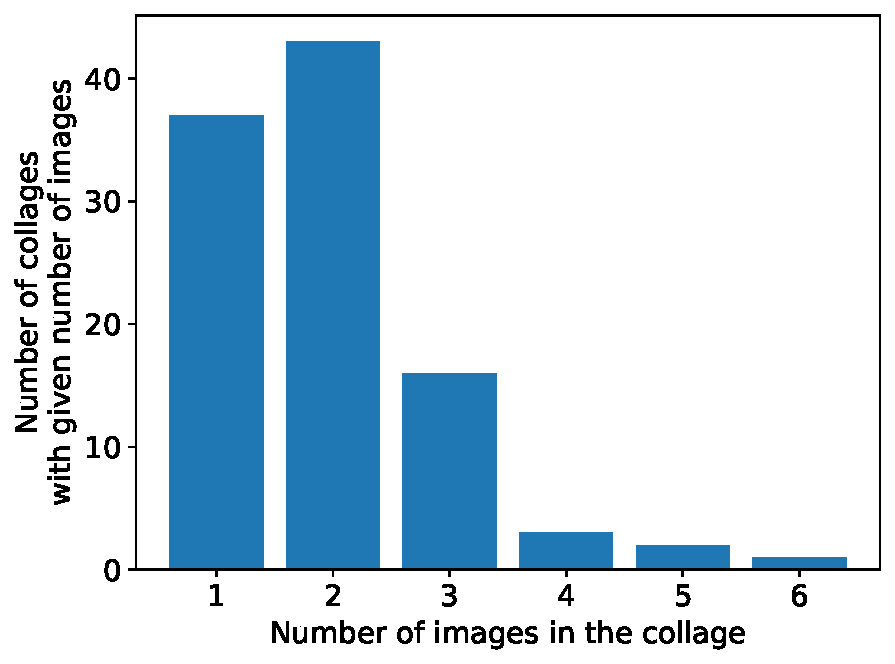
\includegraphics[width=\textwidth]{graphs/num_queries_in_request.pdf}
         \caption{Number of images on a canvas for a collage.}
         \label{fig:y equals x}
     \end{subfigure}
     \hfill
     \begin{subfigure}[b]{0.48\textwidth}
         \centering
         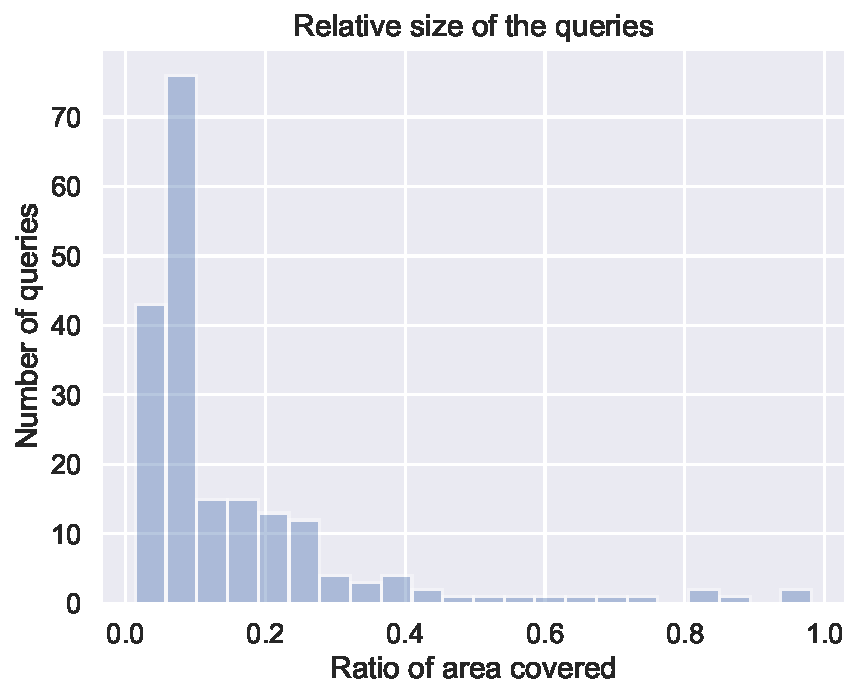
\includegraphics[width=\textwidth]{graphs/queries_size.pdf}
         \caption{Size of the canvas which is covered by a query image.}
         \label{fig:three sin x}
     \end{subfigure}
    
    \caption{Annotated collages properties}
    \label{fig:annotated_dataset}
\end{figure}

\section{Task formulation and evaluations overview}

In our task, we have a dataset $D$ of images and a target image $t$. Since we work with a known-item search task, we know that a target image $t$ is also present in the dataset. Our goal is to create a query $q$, to which the most similar image from the dataset is the target image. We extrapolate the from yes-no on the question "is the target image the most similar image to the query" to "if the results are ordered based on the similarity, at which position is our target image?". We order the items in the dataset so that the images on the lowest position (zero is the best, the most similar) have the highest similarity to the query. We refer to the position of our target image $t$ in such ordering as $rank_{q,D}(t)$ given query $q$ and dataset $D$. The range of the $rank_{q,D}(t)$ function is $[0, |D|)$.

Our goal is to develop a technique that minimizes the target image's rank, given the query. In the following chapters, we aim to test two different possibilities for query description, and we compare their performance based on their ability to retrieve the target image.

So far, we talked only about one query and one target image. We generalize the results from multiple queries by producing a cumulative summary. For each query coupled with the target image, we obtain the $rank_{q, D}(t)$. Then, we can measure the queries' success rate, as the number of queries solved up to a given rank. For example, let us have 40 items in the dataset and perform five queries. These queries ranked the target image at the following positions: \{0, 23, 7, 14\}. For a given rank, we are interested in, we compute how many queries were ranked below it. In this scenario, for a rank 20, three queries were ranked lower.

Since the size of the dataset and the number of tested queries may vary, we always present the results with respect to the size of the set it comes from. In the previous scenario, 75\% of the queries were ranked below the rank representing 50\% of the dataset.

We use these cumulative, proportional results to plot the performance of the framework. A sample evaluation is present in the figure \ref{fig:mobilenet_whole_image_example}. In the case described presented, 90\% of the annotated collages (queries), the target image was ranked in the first 50\% of the dataset. In other words, this can be said that in 90\% of cases by stating a query, we were able to eliminate half of the dataset as unrelated. We can also notice a steep curve in the beginning. It shows that 70\% of the collages had the target image ranked in the first 10\% of the dataset. We can see that this particular system worked well for 70\% of the collages, but struggled to solve the rest.

\begin{figure}
    \centering
    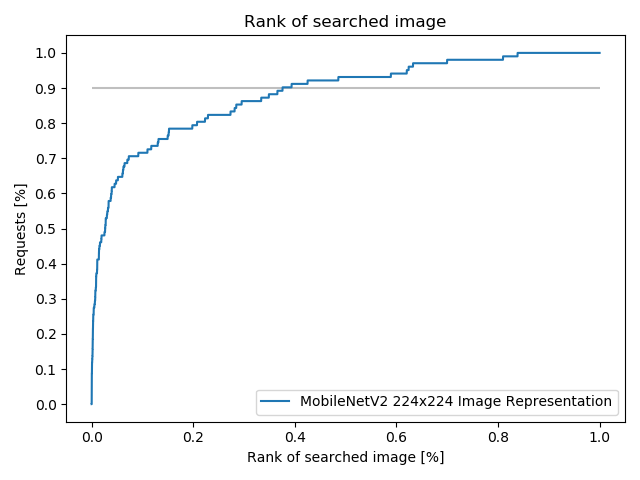
\includegraphics[width=0.8\linewidth]{img/mobilenet_whole_image.png}
    \caption{Performance of MobileNetV2 on annotated collages}
    \label{fig:mobilenet_whole_image_example}
\end{figure}

For these evaluations, we use annotated queries. We described them in section \ref{s:dataset}.

\section{Distance Measures}

In the next chapters, we often compare two high-dimensional feature vectors. These vectors are often produced as a prediction of a neural network. Our feature space is $\mathbb{R}^n$, given $n$ as the number of features. We search for a distance measure function $d: \mathbb{R}^n \times \mathbb{R}^n \rightarrow \mathbb{R}$. We use the following three:

\subsection{Euclidean Distance}

For given $\bf{p}, \bf{q} \in \mathbb{R}^n$ we compute the distance as:
\begin{equation}
d_e({\bf p},{\bf q}) = \sqrt{\sum_{i=1}^n (p_i - q_i)^2}    
\end{equation}


\subsection{Manhattan Distance}

For given $\bf{p}, \bf{q} \in \mathbb{R}^n$ we compute the distance as:
\begin{equation}
d_m({\bf p},{\bf q}) = {\sum_{i=1}^n |p_i - q_i|}    
\end{equation}


\subsection{Cosine Distance}

For given $\bf{p}, \bf{q} \in \mathbb{R}^n$ we compute the distance as:
\begin{equation}
\text{similarity}({\bf p},{\bf q}) = \cos ({\bf p},{\bf q})= {{\bf p} {\bf q} \over \|{\bf p}\| \|{\bf q}\|} = \frac{ \sum_{i=1}^{n}{p_i q_i} }{ \sqrt{\sum_{i=1}^{n}{p_i^2}} \sqrt{\sum_{i=1}^{n}{q_i^2}} }
\end{equation}

\begin{equation}
    d_{cos}({\bf p},{\bf q}) = 1 - \text{similarity}({\bf p},{\bf q})
\end{equation}